%\documentclass{article}
%\usepackage{graphicx,subfigure}
%\begin{document}

\begin{figure}[!h]
  \centering
  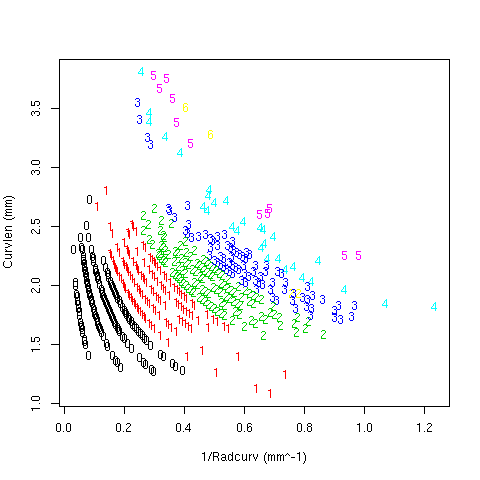
\includegraphics[width=1.0\textwidth]{curvxcurvlenxh.png}
  \caption{Plot of  1/Radius of curvature against curved length of follicles. The sagitta height (h) is shown as point labels which are sagitta height scaled by 10}
  \label{fig:curvxcurvlenxh}
\end{figure}

%\end{document}

